\chapter{Marco Conceptual}

\section{Realidad virtual}
Algunos autores definen así la Realidad Virtual.\\
\newline
\textit{“La realidad virtual (RV) es una simulación tridimensional generada o asistida comúnmente por computadora de algún aspecto del mundo real o ficticio, en el cual 
el usuario tiene la sensación de pertenecer a ese ambiente sintético o interactuar con él”}\cite{web6}\\ 
\textbf{Corrado Padila Érica}\\
\newline
“Realidad Virtual: gráficos 3D en entornos inmersivos que usan I/O
artefactos como guantes, cascos, etc. en busca de mayores grados de iteración
con el ambiente virtual”\cite{web7}\\ 
\textbf{Lozano Miguel, Calderón}\\
\newline
"Realidad Virtual es una forma en que los seres humanos puedan
visualizar, manipular e interactuar con las computadoras y datos extremadamente
complejos".\cite{web8}\\
\textbf{Isdale, Jerry}\\
\newline
“Un sistema interactivo capaz de crear una simulación que implique a varios de los sentidos del ser humano, generados por una computadora, explorable, visualizable y manipulable 
en tiempo real; este bajo la forma de imágenes y sonidos, estos, dando la sensación de presencia en el entorno generado”\cite{web9}\\
\textbf{Levis, Diego}\\
\newline
Esta última ha sido la definición que se ha tomado para el desarrollo del proyecto del trabajo terminal, asimismo se puede concluir que todos los autores coinciden en que la 
realidad virtual es un mundo simulado en el que el usuario puede interactuar en tiempo real por medio
de dispositivos o computadoras que logran un efecto artificial e inmersivo en el que se pueden manipular objetos.

\section{Relaidad Virtual como Apoyo a la Enseñanza-Aprendizaje}%Algo breve de lo que ya se tiene


\section{El sistema digestivo}

\section{Modelos 3D de lo Organos}
En general, independientemente de la disciplina, el proceso de modelado es una simplificación de un objeto para su posterior estudio o representación. Así, podemos hablar de modelos matemáticos que simplifican fenómenos físicos, o modelos meteorológicos para la predicción del tiempo atmosférico, etc. Un modelo geométrico define la información sobre la forma (geometría) de un determinado objeto. Las simplificaciones que se realicen en su definición vendrán determinadas por diferentes factores como el método de representación utilizado, operadores empleados o nivel de detalle.\cite{web13} \\

Se puede definir el proceso de modelado geométrico tridimensional como el encargado de crear modelos consistentes que puedan ser manejados algorítmicamente en un computador. Este proceso de construcción se aborda en diferentes etapas, partiendo típicamente de entidades básicas y aplicando una serie de operadores sobre ellas. Estas entidades básicas pueden ser primitivas geométricas (calculadas de forma algorítmica o mediante una ecuación matemática) u obtenidas mediante un dispositivo de captura (escáner 3D).\\

Existen multitud de técnicas de modelado 3D. En una primera taxonomía de alto nivel podemos hacer una categorización dependiendo de si el modelado se centra en definir únicamente las características del contorno del objeto, los siguiente son los mas usados:\\
\begin{itemize}
\item \textbf{Modelado Sólido:} también conocidos como de Geometría Sólida Constructiva (CSG Constructed Solid Geometry). Los modelos sólidos definen el volumen del objeto que representan, y en muchos casos indican incluso el centro de masas, la densidad del material interna, etc. Se utilizan en fabricación por computador y en aplicaciones médicas e industriales.
\item \textbf{Modelado de Contorno:} también conocidos como de Representación de Contorno (B-Rep - Boundary Representation). Los modelos de contorno únicamente representan la superficie límite del objeto (de forma conceptual, la "cáscara"). Son más fáciles de definir y modificar. Además, lo interesante para la representación del objeto es su apariencia exterior (en los casos donde interesa el interior simplemente se aproxima, como en el caso del SubSurfaceScattering). Prácticamente todos los paquetes de diseño y animación (incluido Blender) empleados en síntesis de imagen y en aplicaciones interactivas emplean este tipo de modelos.
\end{itemize}
Para  cubrir las necesidades de los modelos 3D de los órganos del sistema digestivo se ha opto por que estos fueran realizados en el modelado de contorno por su facilidad de desarrollo y ligereza de carga en el renderizado en el momento de la implementación de estos en el sistema de realidad virtual.\\

\section{Generacion de Entorno 3D}
El entorno 3D es en donde el usuario se encontrará al ingresar al sistema de realidad virtual, para, este se ha realizado para dar la sensación de encontrarse en un ambiente médico.\\

Se utilizaron modelos ya realizados por un autor adquiriendo los derechos de uso ya que la realización de estos no se consideran parte integral del desarrollo del Trabajo Terminal, escrito esto no se quiere demeritar la necesidad de hacer el usuario ya que, como se ha mencionado en secciones anteriores, se tiene énfasis en la experiencia del usuario para que la inmersión del usuario sea la mayor posible.\\

A continuación se muestran capturas del entorno 3D como fue implementado dentro el motor de desarrollo Unity.\\

\begin{figure}[H]
	\begin{center}
 		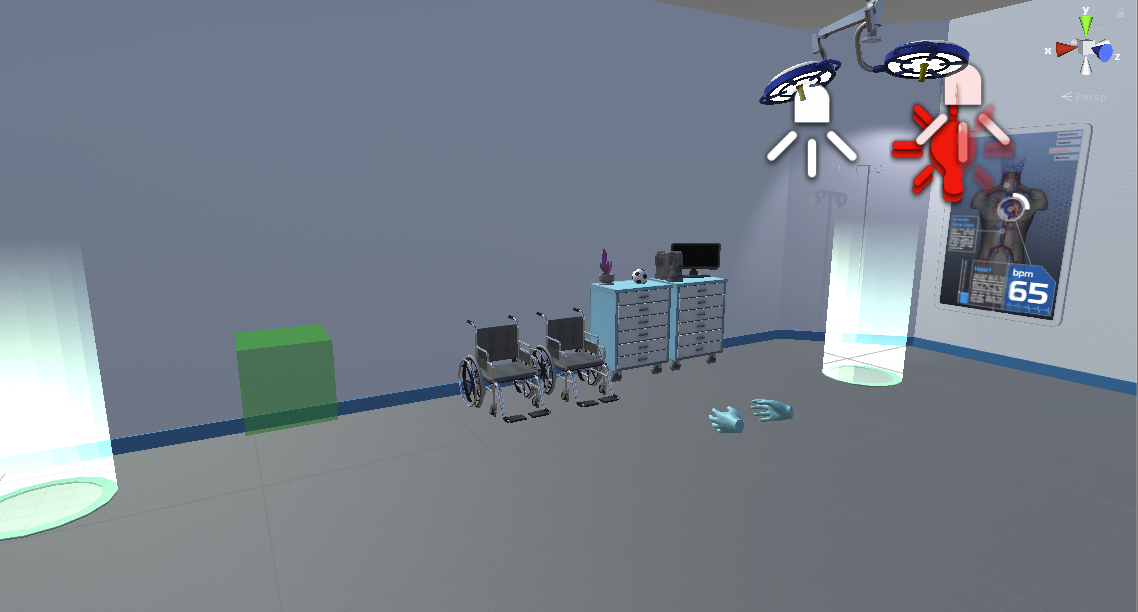
\includegraphics[width = .5\textwidth]{source/images/image63.png}
 		\captionof{figure}{\label{fig:im31}Entorno 3D vista normal}
	\end{center} 
\end{figure}

\begin{figure}[H]
	\begin{center}
 		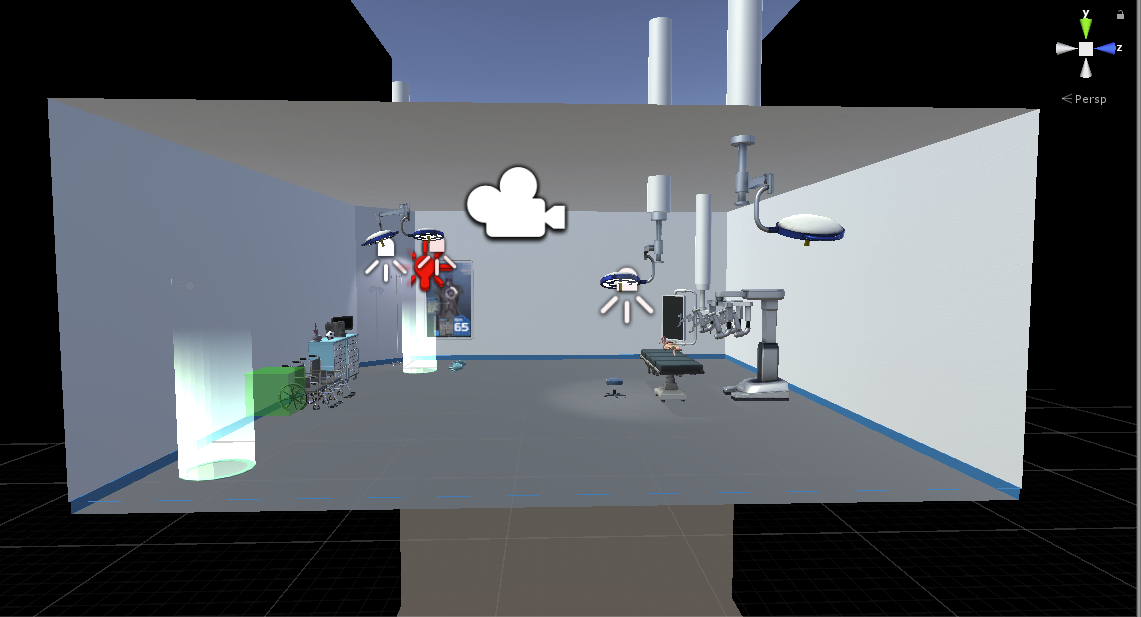
\includegraphics[width = .5\textwidth]{source/images/image53.png}
 		\captionof{figure}{\label{fig:im32} Entorno 3D vista externa de la escena}
	\end{center} 
\end{figure}

\begin{figure}[H]
	\begin{center}
 		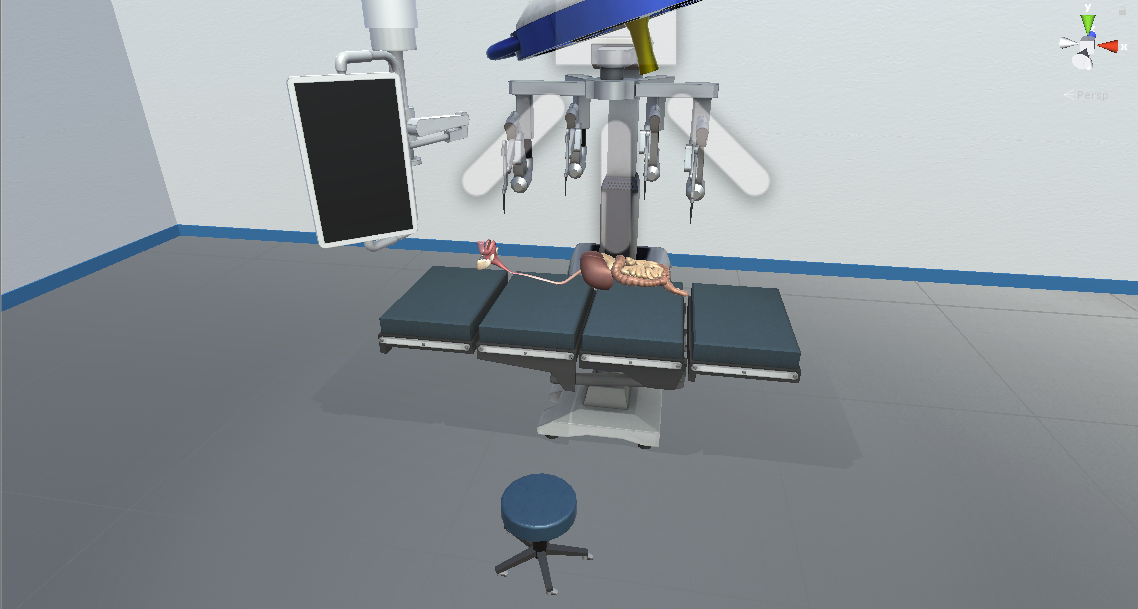
\includegraphics[width = .5\textwidth]{source/images/image16.png}
 		\captionof{figure}{\label{fig:im33}Entorno 3D  vista principal}
	\end{center} 
\end{figure}

\section{Generacion de Modelos 3D}
Los componentes multimedia a desarrollar en modelos 3D los cuales son miembros del sistema digestivo del ser humano, el sistema digestivo incluye a los órganos del tubo alimenticio y glándulas de secreción exocrina y endocrina.\\

\subsection{Glándulas Salivales}
A continuación se muestran las figuras del resultado final del desarrollo de las glándulas salivales del sistema digestivo en el software de modelado en 3D llamado “Blender”, este fue realizado basado en el material anteriormente provisto.\\
\begin{figure}[H]
	\begin{center}
 		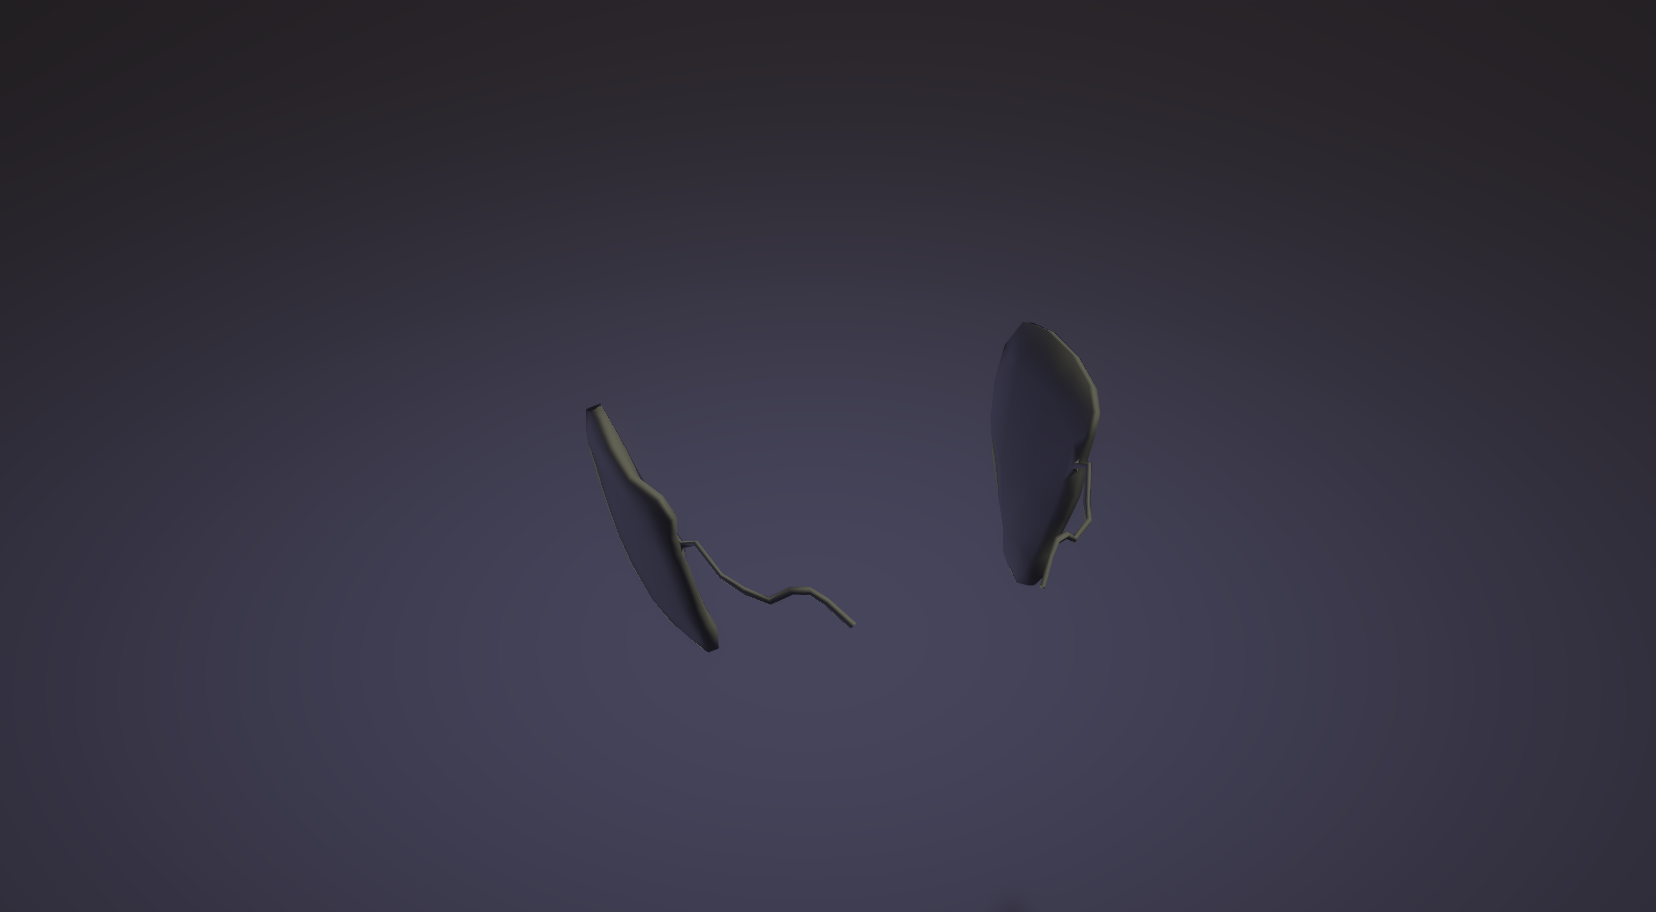
\includegraphics[width = .5\textwidth]{source/images/image41.png}
 		\captionof{figure}{\label{fig:im34}Modelo 3D de las glándulas salivales}
	\end{center} 
\end{figure}

\subsection{Cavidad oral y faringe}
A continuación se muestran las figuras del resultado final del desarrollo de la cavidad oral del sistema digestivo en el software de modelado en 3D llamado “Blender”, este fue realizado basado en el material anteriormente provisto.\\
\begin{figure}[H]
	\begin{center}
 		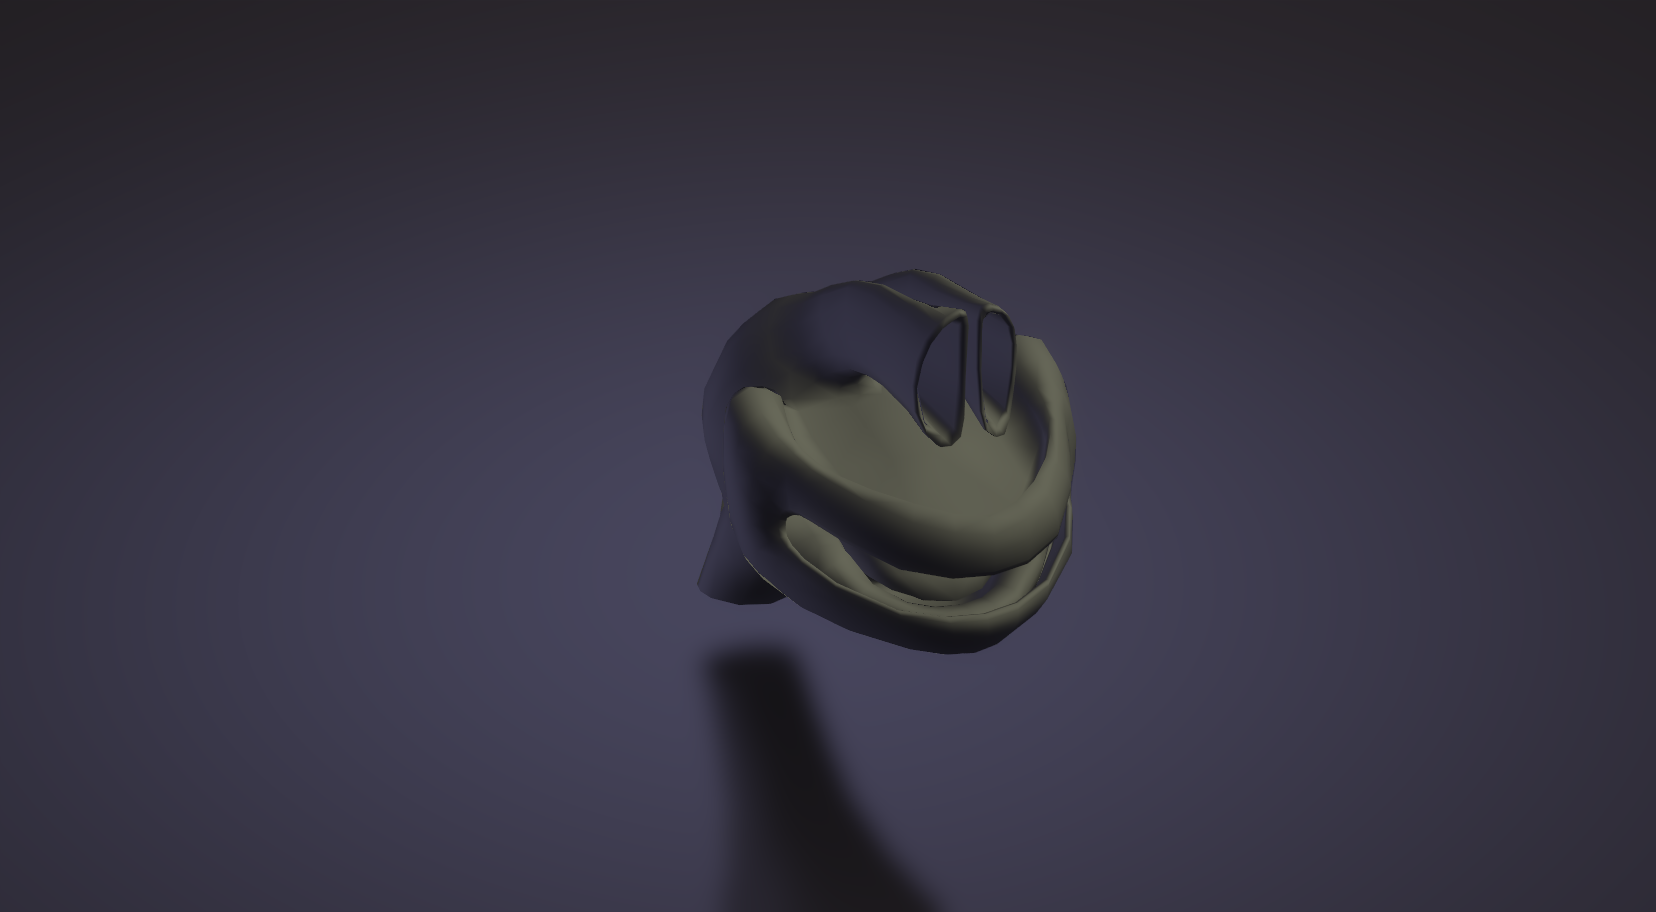
\includegraphics[width = .5\textwidth]{source/images/image14.png}
 		\captionof{figure}{\label{fig:im35}Modelo 3D de la cavidad oral}
	\end{center} 
\end{figure}

\subsection{Esófago}
A continuación se muestran las figuras del resultado final del desarrollo del esófago del sistema digestivo en el software de modelado en 3D llamado “Blender”, este fue realizado basado en el material anteriormente provisto.\\
\begin{figure}[H]
	\begin{center}
 		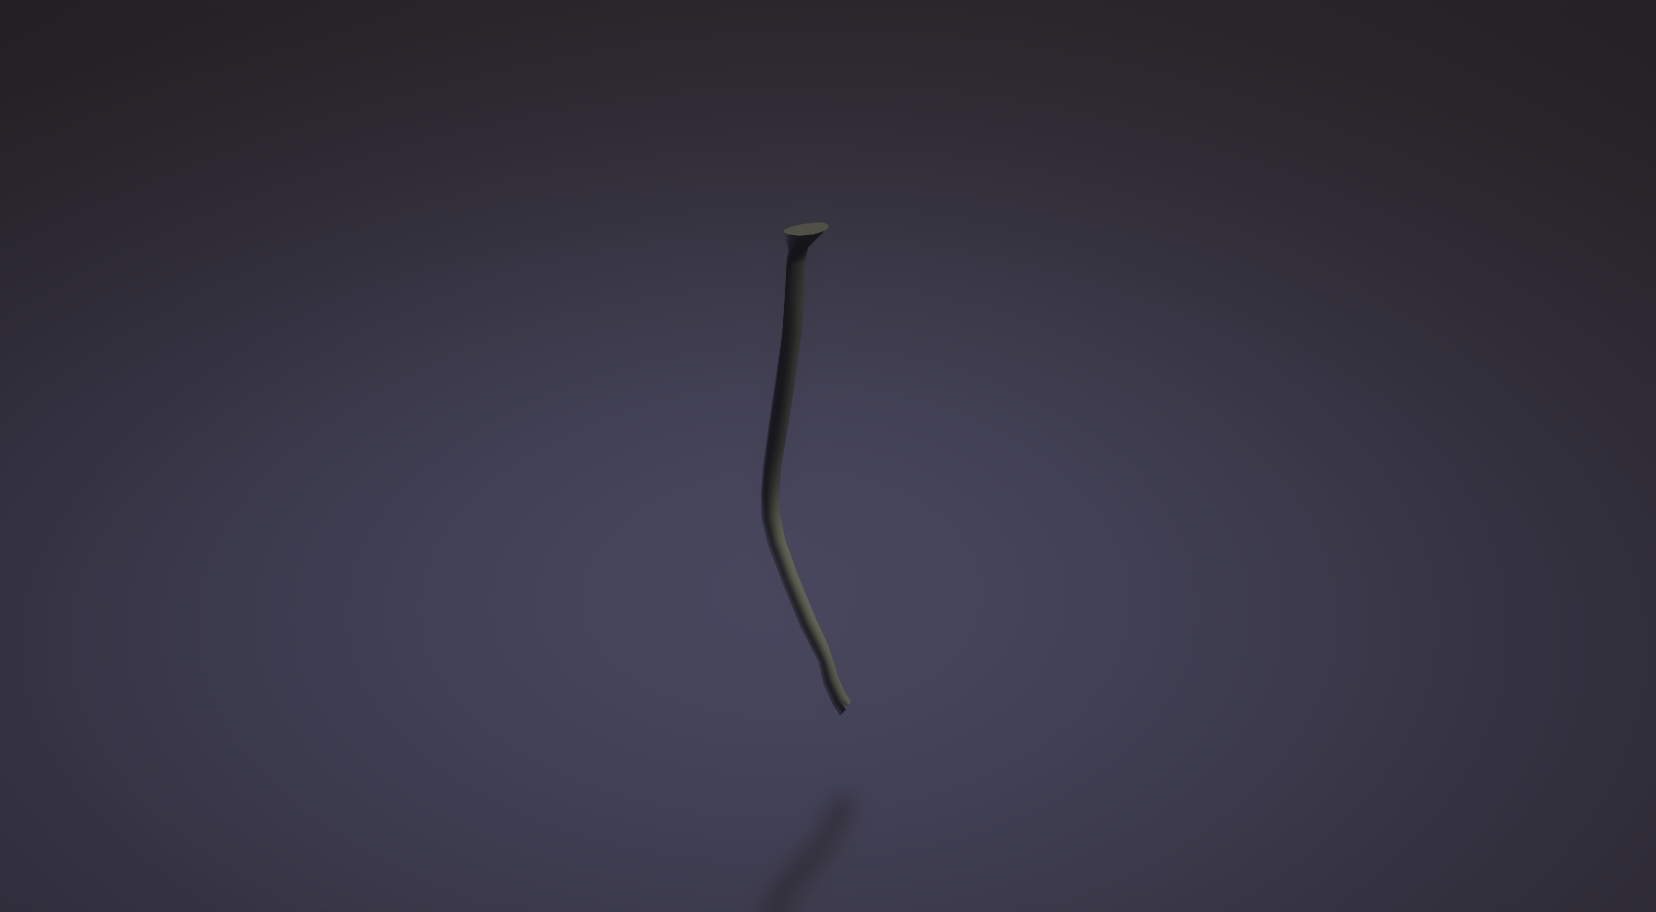
\includegraphics[width = .5\textwidth]{source/images/image25.png}
 		\captionof{figure}{\label{fig:im36}Modelo 3D del esófago}
	\end{center} 
\end{figure}

\subsection{Estómago}
A continuación se muestran las figuras del resultado final del desarrollo del estómago del sistema digestivo en el software de modelado en 3D llamado “Blender”, este fue realizado basado en el material anteriormente provisto.\\
\begin{figure}[H]
	\begin{center}
 		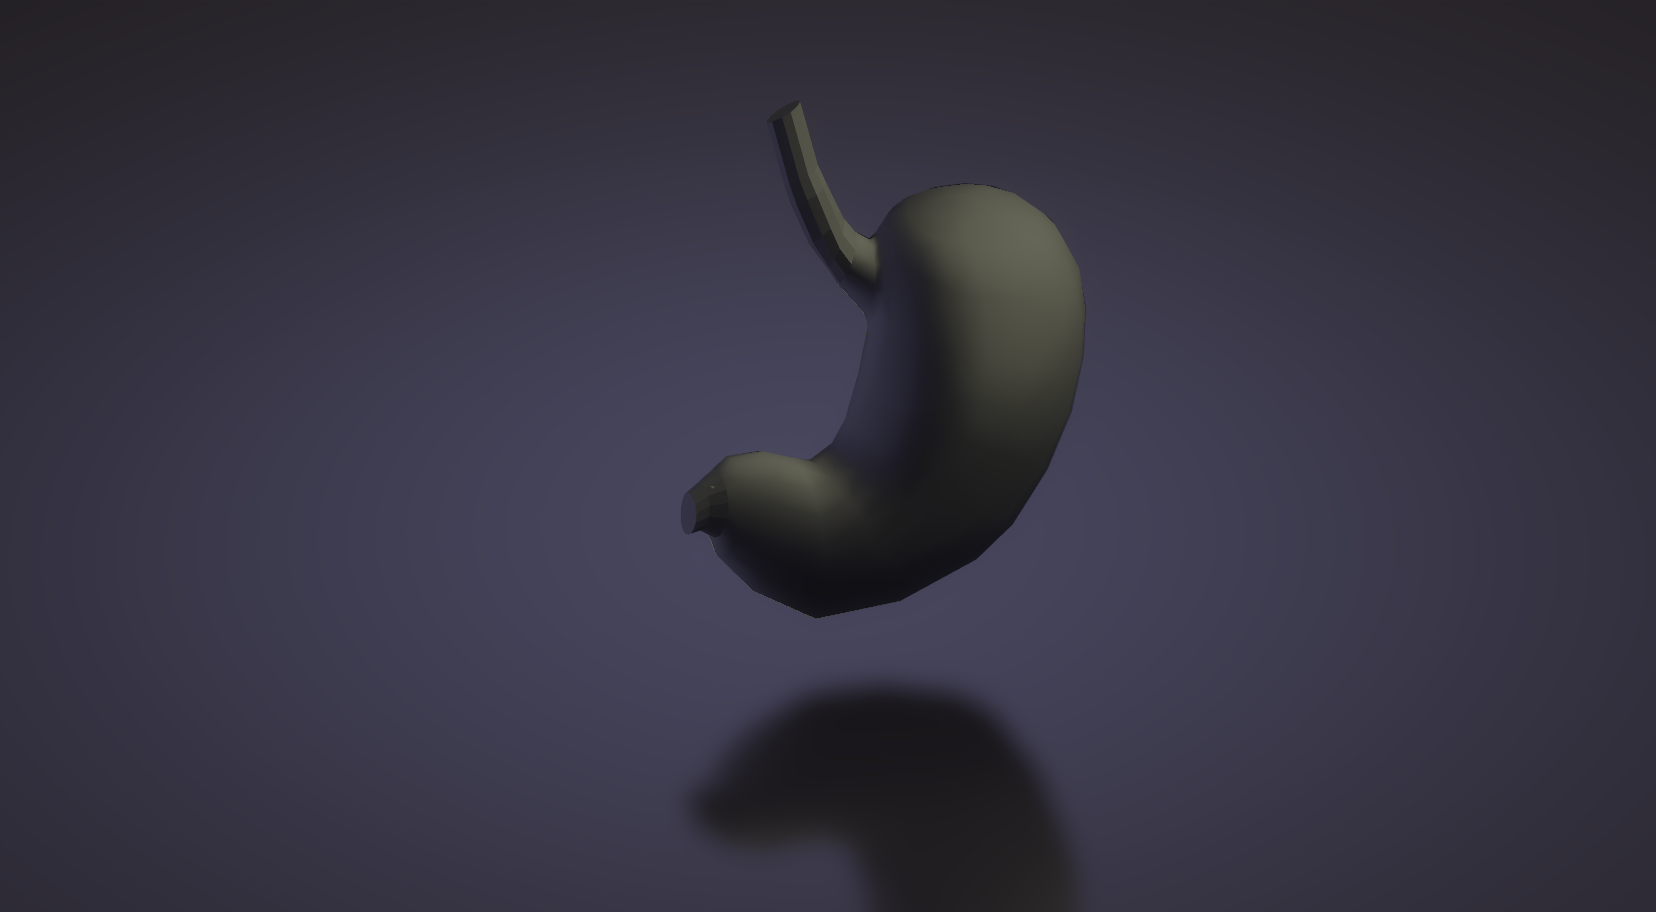
\includegraphics[width = .5\textwidth]{source/images/image42.png}
 		\captionof{figure}{\label{fig:im37} Modelo 3D del estómago }
	\end{center} 
\end{figure}

\subsection{Intestino delgado}
A continuación se muestran las figuras del resultado final del desarrollo del intestino delgado del sistema digestivo en el software de modelado en 3D llamado “Blender”, este fue realizado basado en el material anteriormente provisto.\\
\begin{figure}[H]
	\begin{center}
 		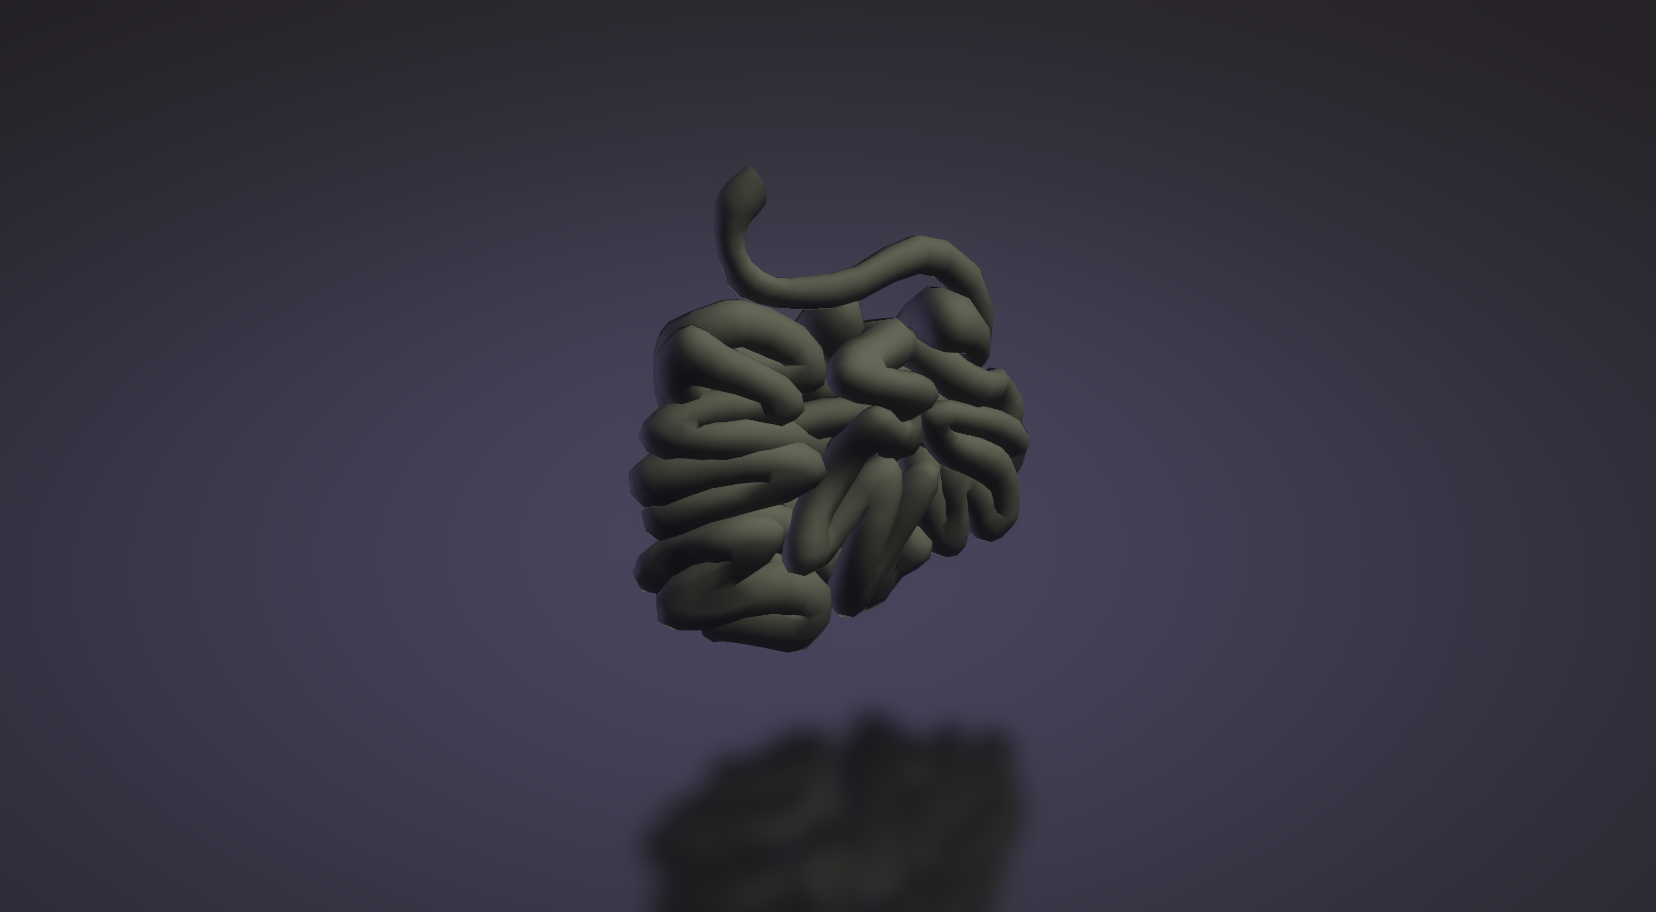
\includegraphics[width = .5\textwidth]{source/images/image69.png}
 		\captionof{figure}{\label{fig:im38}Modelo 3D del intestino delgado}
	\end{center} 
\end{figure}

\subsection{Hígado}
A continuación se muestran las figuras del resultado final del desarrollo del hígado del sistema digestivo en el software de modelado en 3D llamado “Blender”, este fue realizado basado en el material anteriormente provisto.\\
\begin{figure}[H]
	\begin{center}
 		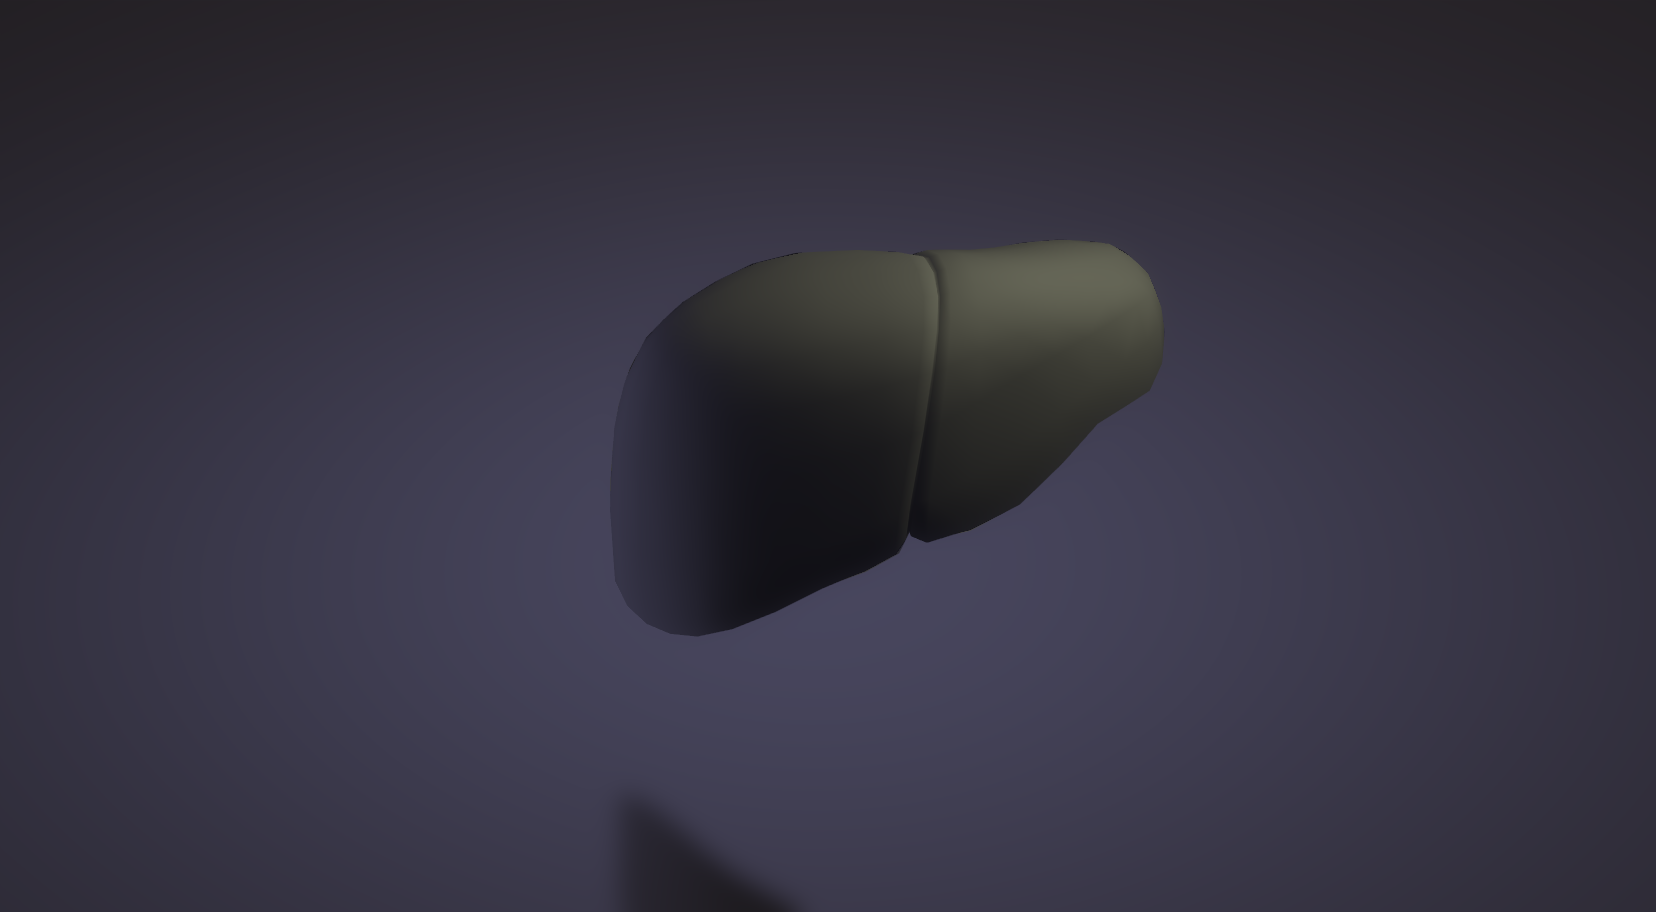
\includegraphics[width = .5\textwidth]{source/images/image17.png}
 		\captionof{figure}{\label{fig:im39}Modelo 3D del hígado}
	\end{center} 
\end{figure}

\subsection{Páncreas}
A continuación se muestran las figuras del resultado final del desarrollo del páncreas del sistema digestivo en el software de modelado en 3D llamado “Blender”, este fue realizado basado en el material anteriormente provisto.\\
\begin{figure}[H]
	\begin{center}
 		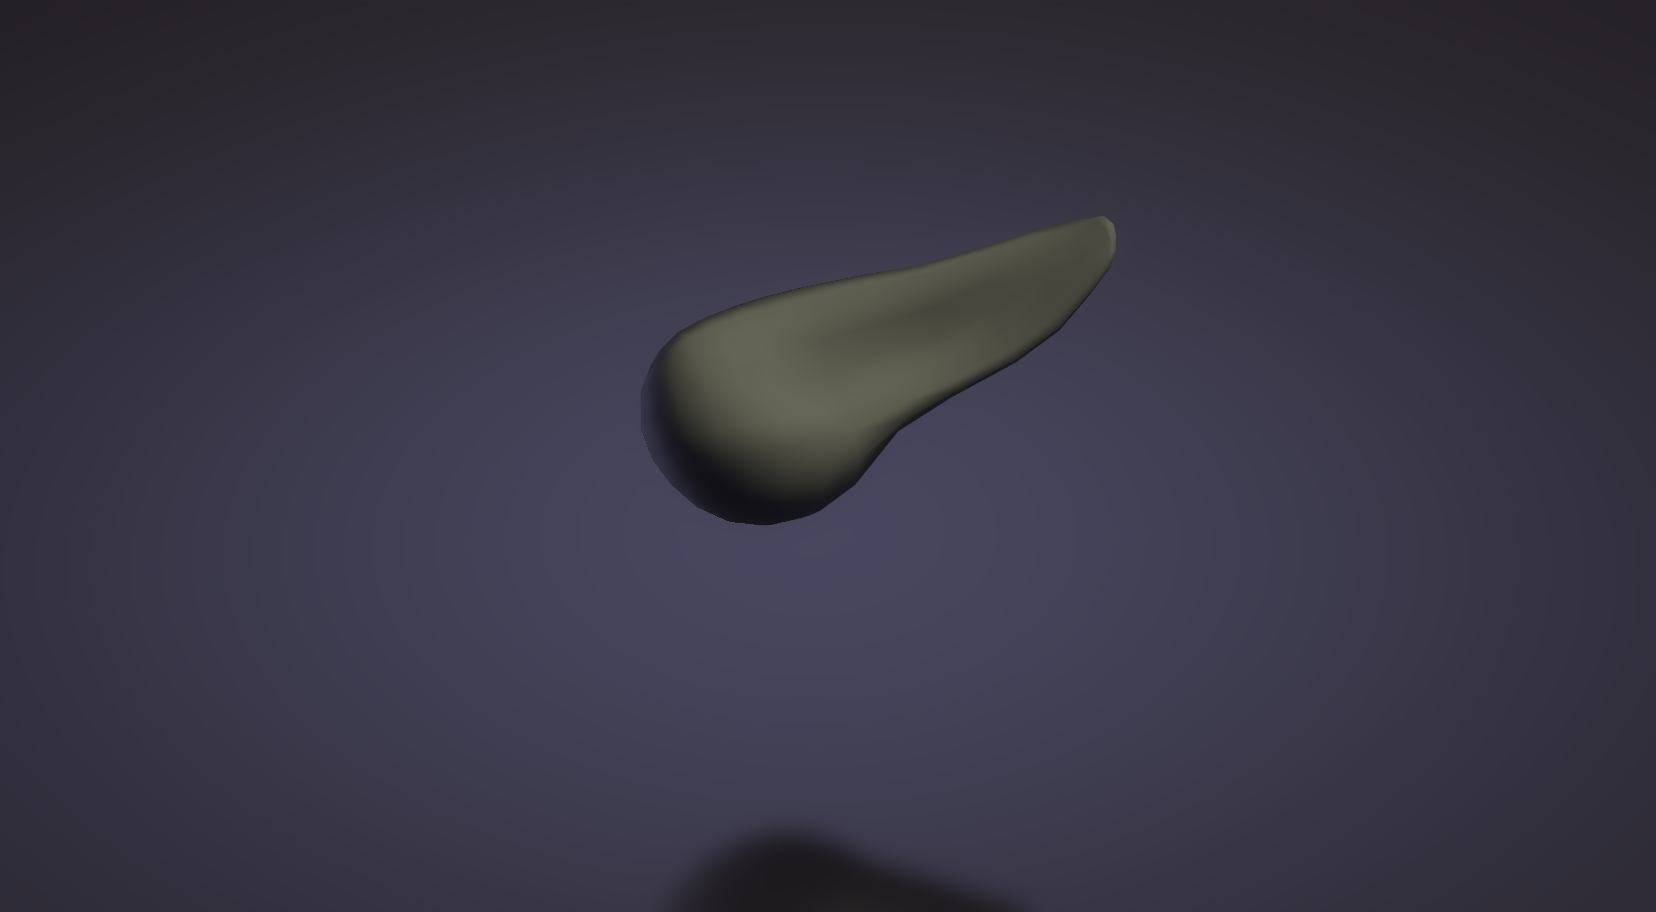
\includegraphics[width = .5\textwidth]{source/images/image19.png}
 		\captionof{figure}{\label{fig:im310}Modelo 3D del páncreas}
	\end{center} 
\end{figure}

\subsection{Vesícula Biliar}
A continuación se muestran las figuras del resultado final del desarrollo de la vesícula biliar del sistema digestivo en el software de modelado en 3D llamado “Blender”, este fue realizado basado en el material anteriormente provisto.\\
\begin{figure}[H]
	\begin{center}
 		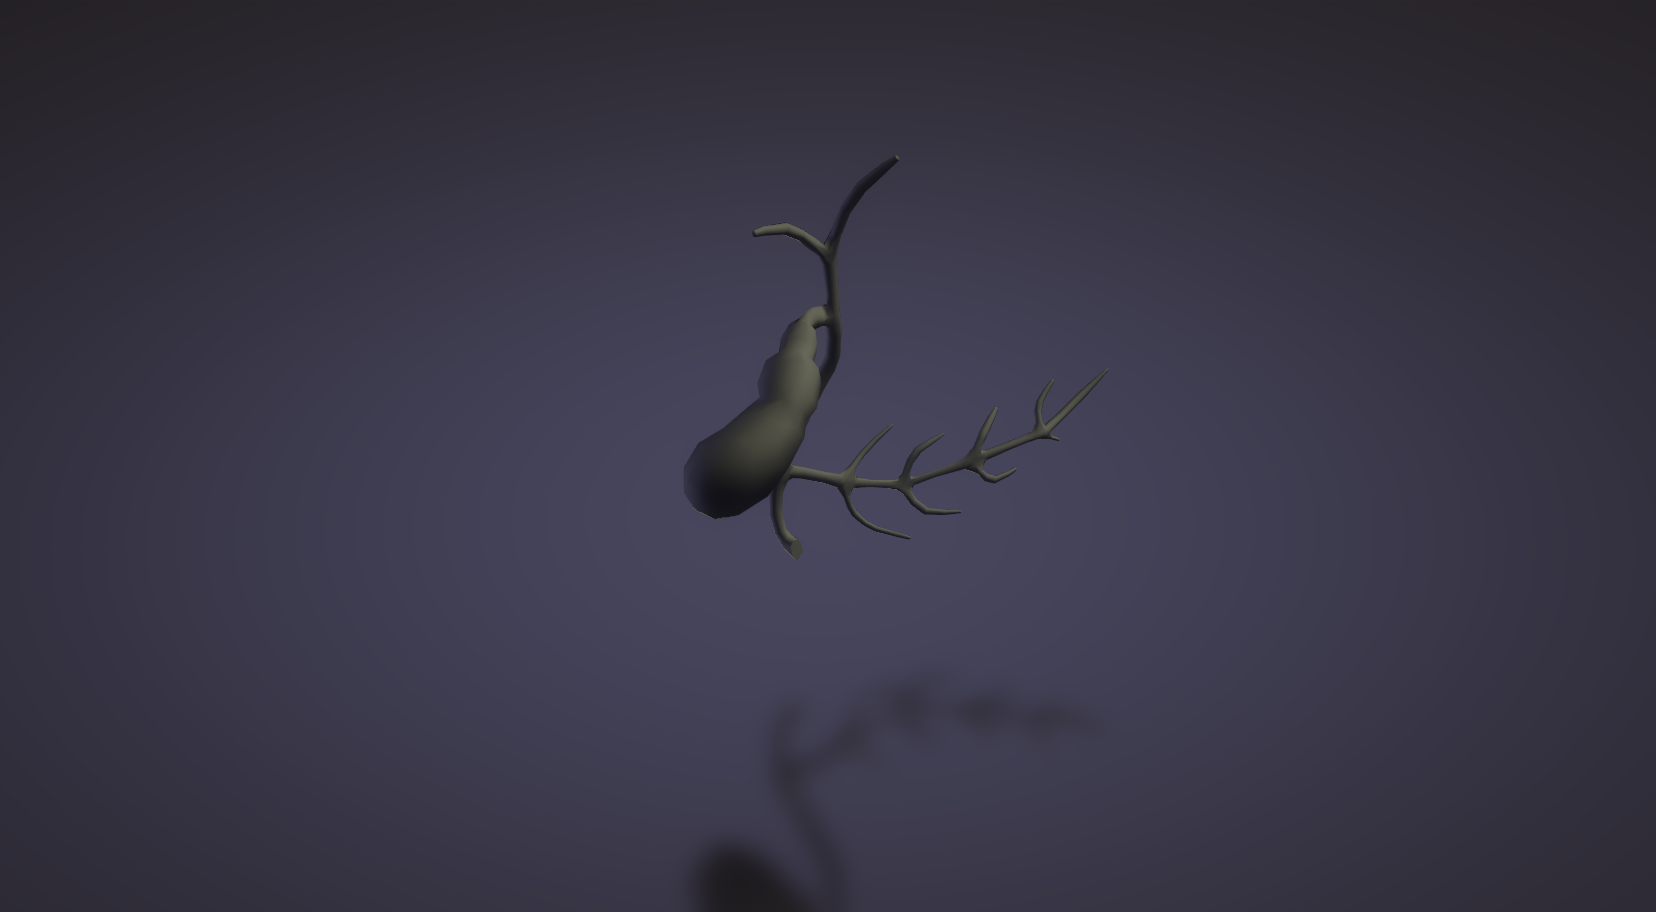
\includegraphics[width = .5\textwidth]{source/images/image26.png}
 		\captionof{figure}{\label{fig:im312}Modelo 3D de la vesícula biliar}
	\end{center} 
\end{figure}

\subsection{Intestino Grueso y Ano}
A continuación se muestran las figuras del resultado final del desarrollo del intestino grueso y ano del sistema digestivo en el software de modelado en 3D llamado “Blender”, este fue realizado basado en el material anteriormente provisto.\\
\begin{figure}[H]
	\begin{center}
 		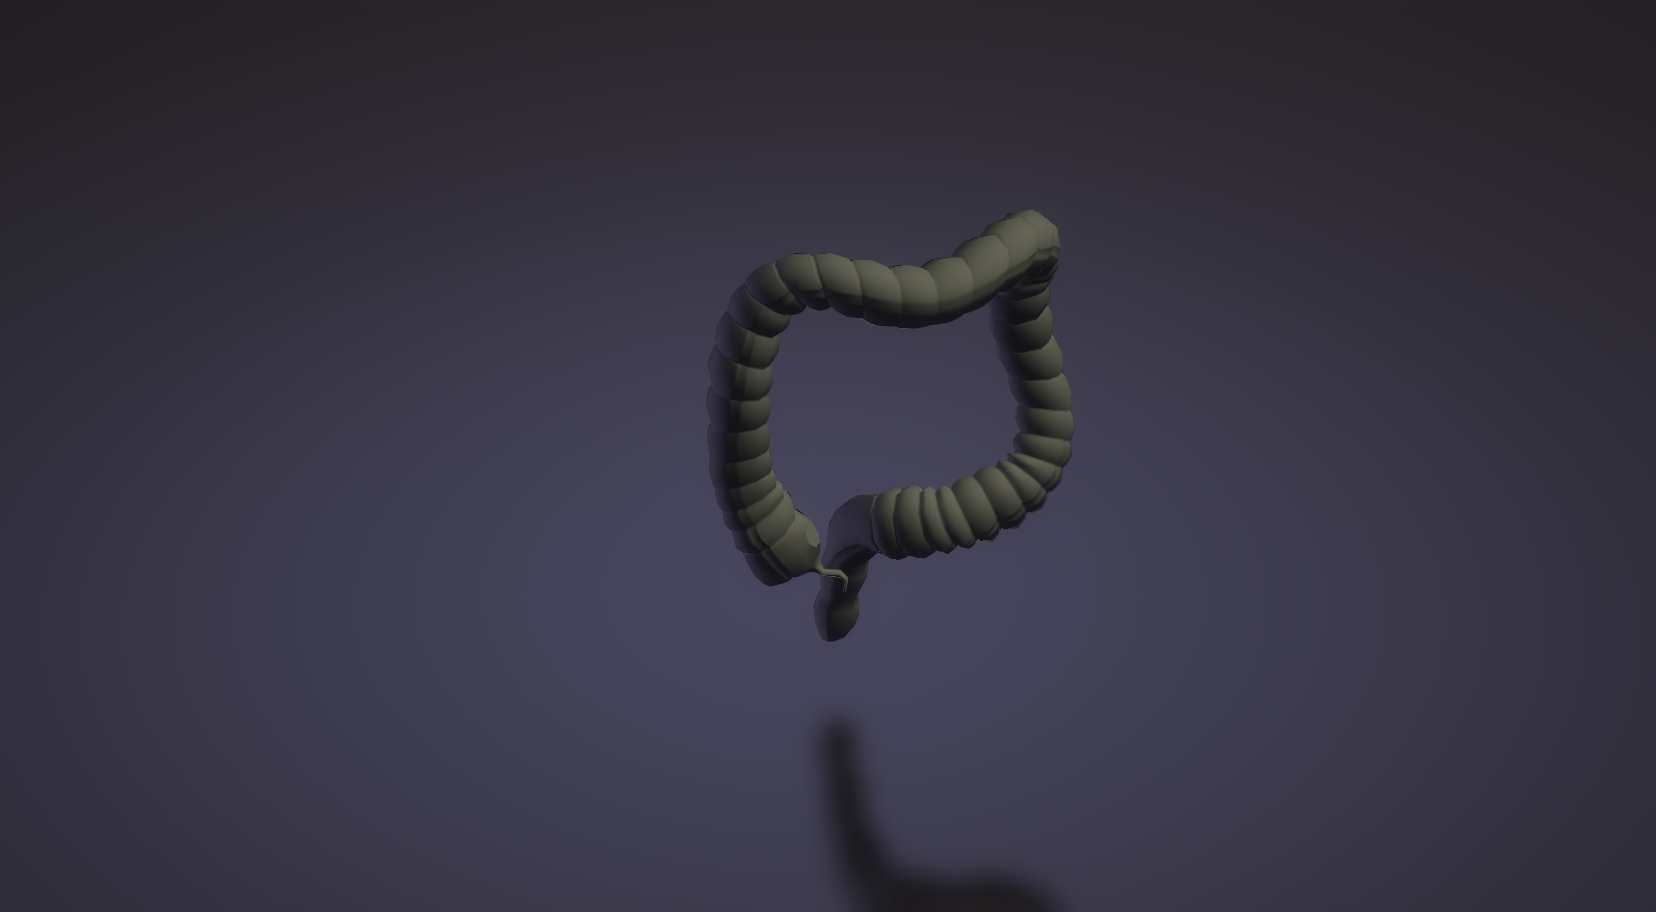
\includegraphics[width = .5\textwidth]{source/images/image20.png}
 		\captionof{figure}{\label{fig:im313}Modelo 3D del intestino grueso}
	\end{center} 
\end{figure}

\section{Modelo del sistema digestivo unificado}
A continuación se muestran las figuras del resultado final del desarrollo del sistema digestivo en el software de modelado en 3D llamado “Blender”, este fue realizado reuniendo todos los modelos de órganos y elementos individuales creados con anterioridad.\\
\begin{figure}[H]
	\begin{center}
 		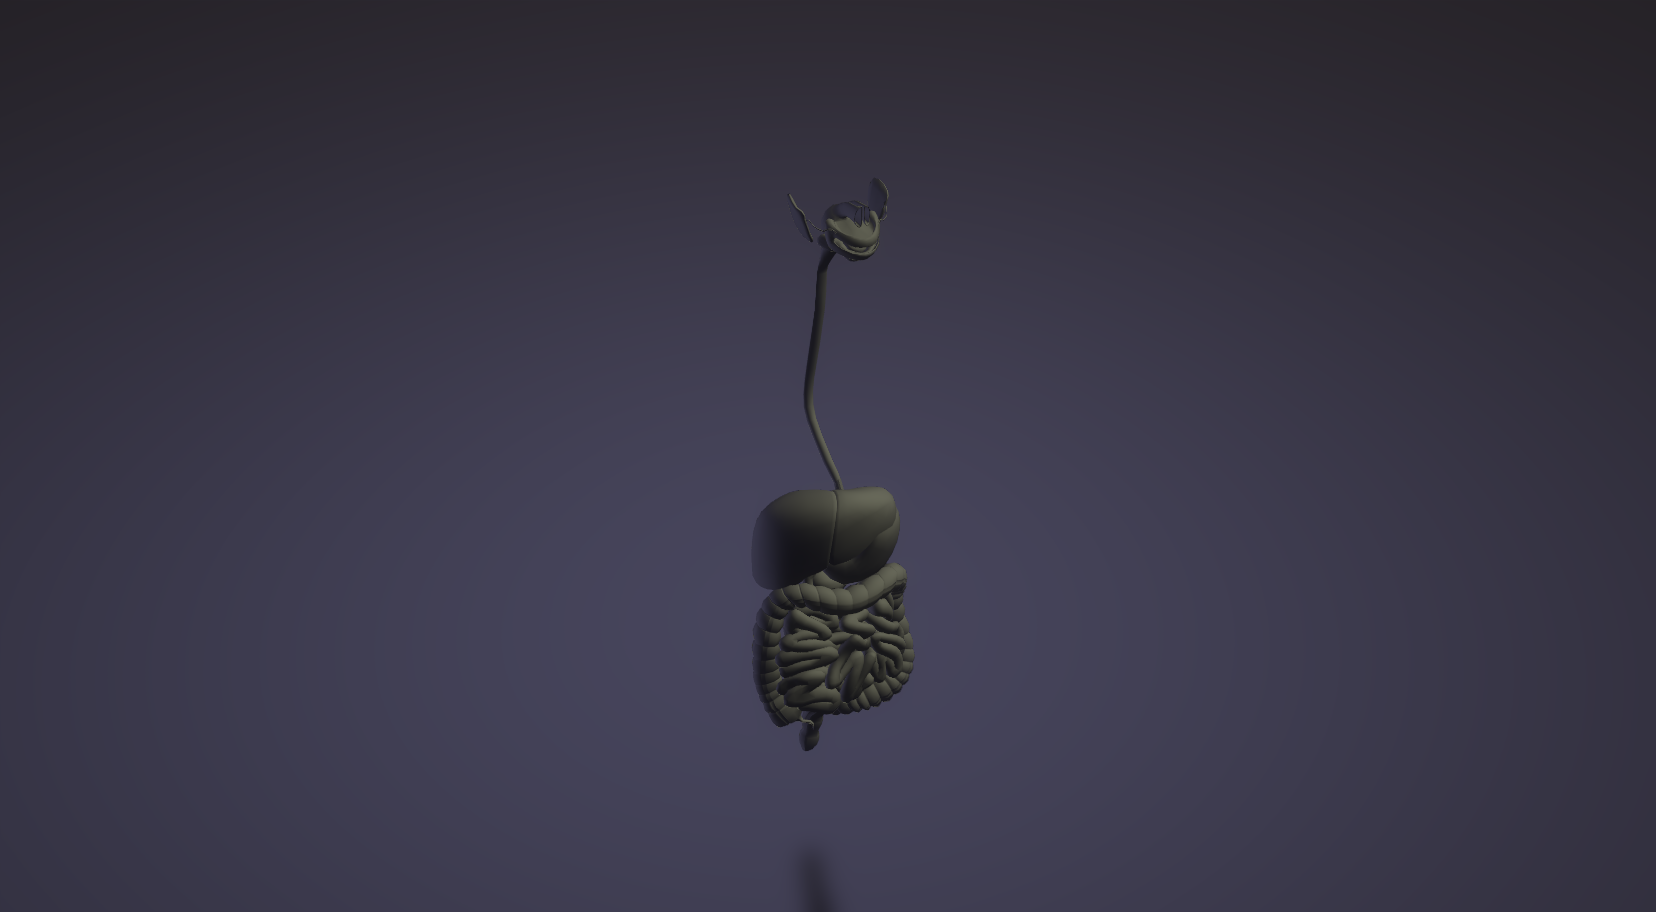
\includegraphics[width = 1\textwidth]{source/images/image24.png}
 		\captionof{figure}{\label{fig:im314}Modelo 3D del Sistema digestivo}
	\end{center} 
\end{figure}

\section{Evaluación de modelos 3D por personal calificado}
Debido al tiempo de desarrollo, el cual tomó más de lo planteado, de los modelos antes expuestos en la sección anterior no fue posible concretar una cita para su evaluación con el personal calificado  de la Escuela Superior de Medicina en las fechas previamente planteadas.\\

Se esperaba poder tener una reunión en fechas posteriores pero la situación epidémica que se ha desarrollado en el país y limitaciones impuestas por las autoridades hicieron imposible la evaluación de los modelos desarrollados.\\

Esto no significa que no se haya hecho bajo rigor alguno, sólo se utilizaron materiales de medicina impresos, así como referencias en video de disecciones del sistema digestivo, esto para estar lo más familiarizado posible, como estudiante de ingeniería en sistemas computacionales, al momento de desarrollar dichos modelos.\\
% (Aquí puede decir lo de unity y demás cosas que se requieren para hacer lo que usted ya hizo)
%(Tratemos de usar lo que se tiene y solo añadir si es indispensable, recortar si es necesario para añadir a Apendices, como lo de las imagenes del aparato digestivo que estaban en el primer documento)